% !TeX encoding = windows-1251
\documentclass[11pt,a4paper]{article}
%\usepackage{russ}
\usepackage[mag=990]{newlistok}
\usepackage{tikz}
\usetikzlibrary{calc}



\УвеличитьШирину{1.8cm}
\УвеличитьВысоту{2.5cm}

\renewcommand{\spacer}{\vfil}

\begin{document}
%\fontsize{11pt}{14pt}
%\selectfont

\Заголовок{Геометрическое суммирование}
\НомерЛистка{1}
\ДатаЛистка{09.2012}


\СоздатьЗаголовок


\задача
Рассмотрим последовательность \лк уголков\пк: $\sDY{1}$\ , $\sDY{2,1}$\ , $\sDY{3,1,1}$\ ,  $\sDY{4,1,1,1}$\ , $\sDY{5,1,1,1,1}$\ ,\ $\ldots$ Сколько клеток в $k$-том уголке и чему равна суммарная площадь первых $k$ уголков?
\кзадача


\задача \пункт Чему равно $k$-е нечётное число и сумма первых $k$ нечётных чисел? \пункт Чему равно $k$-е
чётное число и сумма первых $k$ чётных чисел? \пункт Вычислите сумму 100 последовательных нечётных чисел,~начиная~с~57.
\кзадача

\задача Числа $T_1=1$, $T_2=3$, $T_3=6$, $T_4=10$, $\ldots $ греческий математик Диофант называл {\it треугольными}: \\
$\sDY{1}\ $, $\sDY{2,1}\ $, $\sDY{3,2,1}\ $, $\sDY{4,3,2,1}\ $,\ $\ldots$
{\it Четырёхугольные числа}\ $\sDY{1}\ $, $\sDY{2,2}\ $, $\sDY{3,3,3}\ $, $\sDY{4,4,4,4}\ $,\ $\ldots$ \hbox{ --- это} квадраты. \\
\пункт Сложите из двух последовательных треугольных чисел квадрат.\\
\пункт Что получится при сложении $T_n$ с $T_{n}$?
\пункт Выразите $T_n$ через $n$
\\ (и тем самым получите формулу для суммы $1+2+3+\dots+n$).
\кзадача
\putthere{167mm}{-15mm}{%
    %
    %Картина для сумм треугольных чисел и т.п.
    %
      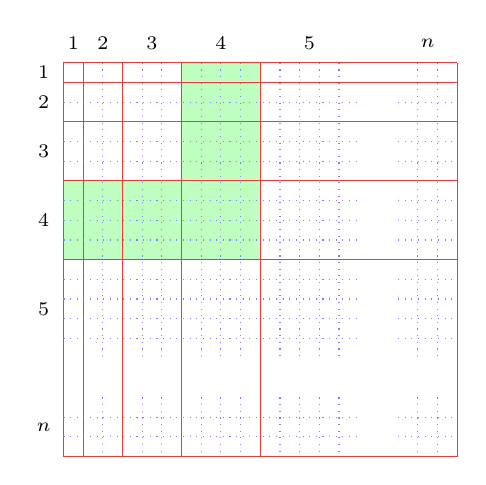
\begin{tikzpicture}
      [scale=.25
      ,fil/.style={color=green!50!white,opacity=.5}
      ,lin/.style={color=red!80}
      ,lindot/.style={color=blue!50,dotted}
      ]
        \fill[fil] (6,0) -- (10,0) -- (10, -10) -- (0,-10) -- (0,-6) -- (6,-6) -- cycle;
        \foreach \i in {0,1,3,6,10,20}{
          \draw[lin] (0, -\i) -- (20, -\i);
          \draw[lin] (\i, 0) -- (\i, -20);
        }
        \foreach \i in {2,4,5,7,8,9,11,12,13,14,18,19}{
          \draw[lindot] (0, -\i) -- (15, -\i);
          \draw[lindot] (17, -\i) -- (20, -\i);
          \draw[lindot] (\i, 0) -- (\i, -15);
          \draw[lindot] (\i, -17) -- (\i, -20);
        }
        \foreach \i in {1,2,...,5}{
          \draw (-1, -\i*\i*.5) node {$\scriptstyle\i$};
          \draw (\i*\i*.5, 1) node {$\scriptstyle\i$};
        }
        \draw (-1, -18.5) node {$\scriptstyle n$};
        \draw (18.5, 1) node {$\scriptstyle n$};
      \end{tikzpicture}
}{7cm}{\risn Пифагорова таблица \\ умножения чисел от 1 до $n$}
\vspace{-4mm}


\задача
Найдите сумму первой сотни натуральных чисел.
\кзадача

\задача Докажите геометрически:
\пункт $T_{m+n}=T_m+T_n+mn$;\\
\пункт $1+2+\dots+(n-1)+n+(n-1)+\dots+2+1=n^2$.
\кзадача

\УстановитьГраницы{0cm}{5.5cm}
\задача[Пифагорова таблица умножения]
\пункт Докажите тождество \\
$mk=km$ (\те докажите, что $\underbrace{k+k+\ldots+k}_m = \underbrace{m+m+\ldots+m}_k$).\\
\пункт Каковы размеры и площадь таблицы на рисунке 1?
\кзадача

\задача
\вСтрочку
\пункт
Сколько клеток в $k$-м, считая от левого верхнего угла
пифагоровой таблицы, \лк толстом\пк\ уголке,
\лк вершина\пк\ которого --- квадрат $k\times k$ клеток, а стороны
составлены из прямоугольников
$1\times k\,,\ 2\times k\,,\ \ldots\,,$ $(k-1)\times k$ клеток\/?
\пункт Найдите сумму $1^3+2^3+\ldots+n^3$.
\кзадача



\putthere{163mm}{-13mm}{%
    %
    % Картинка для пятиугольных чисел
      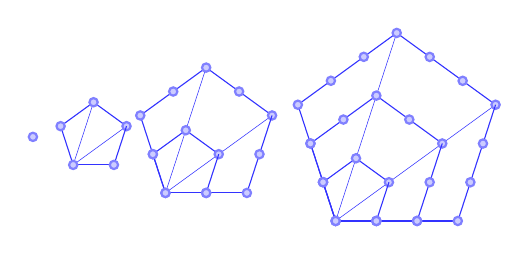
\begin{tikzpicture}
      [scale=.11
      ,ver/.style={circle,draw=blue!50,fill=blue!20,thick,inner sep=0,minimum size=3}
      ,lin/.style={color=blue!80}]
        \coordinate (A0) at (0,0);
        \coordinate (A1) at (7,0);
        \coordinate (A2) at (20,0);
        \coordinate (A3) at (42,0);
        \node[ver] at (A0){};
        \draw[lin,very thin] (A1) + (-126:4) -- +(18:4);
        \draw[lin,very thin] (A1) + (-126:4) -- +(90:4);
        \foreach \a in {18,90,...,306}{
          \draw[lin] (A1)
                                       +(\a:4)    node[ver]{}
                                    -- +(\a+72:4);
        }
        \draw[lin,very thin] (A2) + (-126:8) -- +(18:8);
        \draw[lin,very thin] (A2) + (-126:8) -- +(90:8);
        \foreach \a in {18,90,...,306}{
          \draw[lin] (A2)
                                       +(\a:8)    node[ver]{} coordinate (A)
                                    -- +(\a+72:8)             coordinate (B);
          \node[ver] at  ($ (A)!.5!(B) $){};
          \draw[lin] (A2) ++ (-126:8) ++ (54:4)
                                       +(\a:4)    node[ver]{} coordinate (A)
                                    -- +(\a+72:4)             coordinate (B);
        }
        \draw[lin,very thin] (A3) + (-126:12) -- +(18:12);
        \draw[lin,very thin] (A3) + (-126:12) -- +(90:12);
        \foreach \a in {18,90,...,306}{
          \draw[lin] (A3)
                                       +(\a:12)    node[ver]{} coordinate (A)
                                    -- +(\a+72:12)             coordinate (B);
          \node[ver] at  ($ (A)!.333!(B) $){};
          \node[ver] at  ($ (A)!.666!(B) $){};
          \draw[lin] (A3) ++ (-126:12) ++ (54:8)
                                       +(\a:8)    node[ver]{} coordinate (A)
                                    -- +(\a+72:8)             coordinate (B);
          \node[ver] at  ($ (A)!.5!(B) $){};
          \draw[lin] (A3) ++ (-126:12) ++ (54:4)
                                       +(\a:4)    node[ver]{} coordinate (A)
                                    -- +(\a+72:4)             coordinate (B);
        }
      \end{tikzpicture}
}{7cm}{\risn Пятиугольные числа.}
\vspace{-4mm}
\УстановитьГраницы{0truecm}{6.5truecm}



\задача
Сформулируйте и докажите теорему, описывающую явление: \\
$3+5=2^3$,~$7+9+11=3^3$,~$13+15+17+19=4^3$,~$\ldots$
\кзадача

\задача
{\it Пятиугольные числа} $P_1=1$, $P_2=5$,
$P_3=12$, $P_4=22$, $\ldots$  показаны на рисунке~2.
Найдите разность $P_k-P_{k-1}$
между последовательными пятиугольными числами.
Выразите $P_n$ через~$n$.
\кзадача

\задача Докажите геометрически, что сумма $n$-го треугольного и $n$-го
четырёхугольного числа на $n$ больше, чем $n$-ое пятиугольное число.
\кзадача


\putthere{169mm}{-11mm}{%
    %
    % пирамидка
      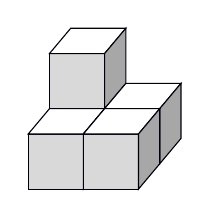
\begin{tikzpicture}
      [scale=.7
    % эти константы задают раскраску граней
      ,fil1/.style={draw=blue!5!black,fill=gray!00,thin}
      ,fil2/.style={draw=blue!5!black,fill=gray!30,thin}
      ,fil3/.style={draw=blue!5!black,fill=gray!69,thin}
      ]
    % эти константы задают наклон кубика
        \coordinate (d) at (50:.6);

        \coordinate (A) at (0,0);
        \coordinate (md) at ($ (0,0) - (d) $);
        \filldraw[fil2] (A) -- +(1,0) -- +(1,1) -- +(0,1) -- cycle;
        \filldraw[fil1] (A)++(1,1) -- ++(d) -- ++(-1,0) -- ++(md) -- cycle;
        \filldraw[fil3] (A)++(1,1) -- ++(d) -- ++(0,-1) -- ++(md) -- cycle;
        \coordinate (A) at ($(0,-1)+(md)$);
        \filldraw[fil2] (A) -- +(1,0) -- +(1,1) -- +(0,1) -- cycle;
        \filldraw[fil1] (A)++(1,1) -- ++(d) -- ++(-1,0) -- ++(md) -- cycle;
        \filldraw[fil3] (A)++(1,1) -- ++(d) -- ++(0,-1) -- ++(md) -- cycle;
        \coordinate (A) at (1,-1);
        \filldraw[fil2] (A) -- +(1,0) -- +(1,1) -- +(0,1) -- cycle;
        \filldraw[fil1] (A)++(1,1) -- ++(d) -- ++(-1,0) -- ++(md) -- cycle;
        \filldraw[fil3] (A)++(1,1) -- ++(d) -- ++(0,-1) -- ++(md) -- cycle;
        \coordinate (A) at ($(1,-1)+(md)$);
        \filldraw[fil2] (A) -- +(1,0) -- +(1,1) -- +(0,1) -- cycle;
        \filldraw[fil1] (A)++(1,1) -- ++(d) -- ++(-1,0) -- ++(md) -- cycle;
        \filldraw[fil3] (A)++(1,1) -- ++(d) -- ++(0,-1) -- ++(md) -- cycle;
       \end{tikzpicture}
}{5cm}{\risn Пирамида для $1^2+2^2$}
\vspace{-4mm}
\УстановитьГраницы{0truecm}{4truecm}


\сзадача Число $k^2$ можно представлять себе как объём параллелепипеда
$1\times k\times k$, а~сумму $1^2+2^2+\ldots+n^2$ --- как объём пирамиды,
сложенной из таких параллелепипедов. Будем обозначать эту пирамиду $Sq(n)$
(на рисунке 3 изображена пирамида $Sq(2)$ объёмом $1^2+2^2$).
Сложите из шести пирамид $Sq(n)$ параллелепипед.
Каковы его размеры и объём? Выведите
формулу для суммы $1^2+2^2+\ldots+n^2$.
\кзадача




\putthere{165mm}{-17mm}{%
    %
    % пирамидки
      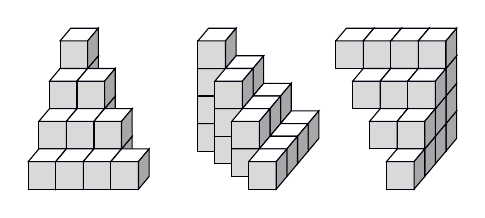
\begin{tikzpicture}
      [scale=.35
      ,fil1/.style={draw=blue!5!black,fill=gray!00,thin}
      ,fil2/.style={draw=blue!5!black,fill=gray!30,thin}
      ,fil3/.style={draw=blue!5!black,fill=gray!69,thin}
      ]
        \coordinate (d) at (50:.6);
        \coordinate (A1) at (0,0);
        \coordinate (A2) at (5,0);
        \coordinate (A3) at (10,0);
        \coordinate (md) at ($ (0,0) - (d) $);

        \foreach \x/\y/\z in {1/4/3, 1/4/4, 2/3/2, 1/3/3, 2/3/3, 3/2/1, 1/2/2, 2/2/2, 3/2/2, 1/1/1, 2/1/1, 3/1/1, 4/1/1}
        {
            \coordinate (A) at ($ (A1) + \x*(1,0) + \z*(0,1) + \y*(d)$);
            \filldraw[fil2] (A) -- +(1,0) -- +(1,1) -- +(0,1) -- cycle;
            \filldraw[fil1] (A)++(1,1) -- ++(d) -- ++(-1,0) -- ++(md) -- cycle;
            \filldraw[fil3] (A)++(1,1) -- ++(d) -- ++(0,-1) -- ++(md) -- cycle;
        }

        \foreach \x/\y/\z in {1/4/1, 1/4/2, 1/4/3, 1/4/4, 2/4/3, 2/3/1, 2/3/2, 2/3/3,   3/4/2, 3/3/2, 3/2/1, 3/2/2,  4/4/1, 4/3/1, 4/2/1, 4/1/1}
        {
            \coordinate (A) at ($ (A2) + \x*(1,0) + \z*(0,1) + \y*(d)$);
            \filldraw[fil2] (A) -- +(1,0) -- +(1,1) -- +(0,1) -- cycle;
            \filldraw[fil1] (A)++(1,1) -- ++(d) -- ++(-1,0) -- ++(md) -- cycle;
            \filldraw[fil3] (A)++(1,1) -- ++(d) -- ++(0,-1) -- ++(md) -- cycle;
        }

        \foreach \x/\y/\z in {4/4/1, 4/3/1, 4/2/1, 4/1/1, 1/4/4, 4/4/2, 4/3/2, 4/2/2, 2/4/4, 3/4/4, 4/4/3, 4/4/4,  2/3/3, 3/3/3, 4/3/3, 3/2/2, 4/2/2}
        {
            \coordinate (A) at ($ (A3) + \x*(1,0) + \z*(0,1) + \y*(d)$);
            \filldraw[fil2] (A) -- +(1,0) -- +(1,1) -- +(0,1) -- cycle;
            \filldraw[fil1] (A)++(1,1) -- ++(d) -- ++(-1,0) -- ++(md) -- cycle;
            \filldraw[fil3] (A)++(1,1) -- ++(d) -- ++(0,-1) -- ++(md) -- cycle;
        }

       \end{tikzpicture}
}{5cm}{\risn Интересные пирамиды}
\vspace{-4mm}
\УстановитьГраницы{0truecm}{6.4truecm}


\задача
\putthere{160mm}{-70mm}{%
    %
    % Таблица
    %
      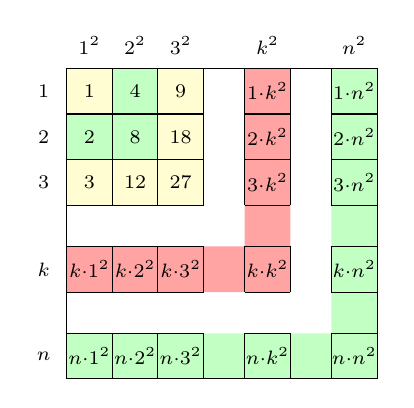
\begin{tikzpicture}
      [scale=.58
      ,fil1/.style={color=green!40!white,opacity=.6}
      ,fil2/.style={color=red!60!white,opacity=.6}
      ,fil3/.style={color=yellow!30!white,opacity=.6}
      ,lin/.style={color=black!100}
      ]
        \fill[fil1] (6.3,-0.5) -- (7.3,-0.5) -- (7.3, -7.3) -- (0.5,-7.3) -- (0.5,-6.3) -- (6.3,-6.3) -- cycle;
        \fill[fil2] (4.4,-0.5) -- (5.4,-0.5) -- (5.4, -5.4) -- (0.5,-5.4) -- (0.5,-4.4) -- (4.4,-4.4) -- cycle;
        \fill[fil3] (2.5,-0.5) -- (3.5,-0.5) -- (3.5, -3.5) -- (0.5,-3.5) -- (0.5,-2.5) -- (2.5,-2.5) -- cycle;
        \fill[fil1] (1.5,-0.5) -- (2.5,-0.5) -- (2.5, -2.5) -- (0.5,-2.5) -- (0.5,-1.5) -- (1.5,-1.5) -- cycle;
        \fill[fil3] (0.5,-0.5) -- (1.5,-0.5) -- (1.5, -1.5) -- (0.5,-1.5) -- cycle;
        \foreach \i in {1.5, 2.5, 3.5, 4.4, 5.4,  6.3}{
          \draw[lin] (0.5, -\i) -- (3.5, -\i);
          \draw[lin] (4.4, -\i) -- (5.4, -\i);
          \draw[lin] (6.3, -\i) -- (7.3, -\i);
          \draw[lin] (\i, -0.5) -- (\i, -3.5);
          \draw[lin] (\i, -4.4) -- (\i, -5.4);
          \draw[lin] (\i, -6.3) -- (\i, -7.3);
        }
        \draw[lin] (0.5, -0.5) -- (0.5, -7.3);
        \draw[lin] (0.5, -0.5) -- (7.3, -0.5);
        \draw[lin] (7.3, -7.3) -- (0.5, -7.3);
        \draw[lin] (7.3, -7.3) -- (7.3, -0.5);
        \draw (1, -1) node {$\scriptstyle 1$};
        \draw (2, -1) node {$\scriptstyle 4$};
        \draw (3, -1) node {$\scriptstyle 9$};
        \draw (1, -2) node {$\scriptstyle 2$};
        \draw (2, -2) node {$\scriptstyle 8$};
        \draw (3, -2) node {$\scriptstyle 18$};
        \draw (1, -3) node {$\scriptstyle 3$};
        \draw (2, -3) node {$\scriptstyle 12$};
        \draw (3, -3) node {$\scriptstyle 27$};
        \foreach \i in {1,2,3}
        {
          \draw (\i, -4.9) node {$\scriptstyle k\cdot\i^2$};
          \draw (4.9, -\i) node {$\scriptstyle\i\cdot k^2$};
          \draw (\i, -6.8) node {$\scriptstyle n\cdot\i^2$};
          \draw (6.8, -\i) node {$\scriptstyle\i\cdot n^2$};
          \draw (\i, 0) node {$\scriptstyle \i^2$};
          \draw (0, -\i) node {$\scriptstyle \i$};
        }

        \draw (4.9, -4.9) node {$\scriptstyle k\cdot k^2$};
        \draw (6.8, -4.9) node {$\scriptstyle k\cdot n^2$};
        \draw (4.9, -6.8) node {$\scriptstyle n\cdot k^2$};
        \draw (6.8, -6.8) node {$\scriptstyle n\cdot n^2$};
        \draw (4.9, 0) node {$\scriptstyle k^2$};
        \draw (6.8, 0) node {$\scriptstyle n^2$};
        \draw (0, -4.9) node {$\scriptstyle k$};
        \draw (0, -6.8) node {$\scriptstyle n$};

      \end{tikzpicture}
}{7cm}{}%{\risn Таблица умножения\\чисел и их квадратов}
На рисунке справа изображены несколько пирамид высоты~4,
каждая из них состоит из $T_1+T_2+T_3+T_4$ кубиков.
\пункт Выберите одну из пирамид на рисунке и нарисуйте её горизонтальные слои:
нижний, второй снизу, \dots , верхний.
\пункт Нарисуйте передний, второй спереди, \dots ,
задний слои выбранной пирамиды;
\пункт Нарисуйте самый левый, второй слева, \dots, самый правый слои выбранной пирамиды.
\пункт Сложите из шести пирамид такого вида параллелепипед. Каковы его размеры?
\ВосстановитьГраницы
\noindent\hspace*{-3.5mm}\пункт Как сложить параллелепипед из шести пирамид аналогичного вида,
но высоты $n$? Найдите формулу для суммы треугольных чисел $T_1+T_2+\dots+T_n$
(эта сумма обозначается $П_n$ и
называется {\it $n$-ым пирамидальным числом}).
\пункт
Сложите из двух таких пирамид высоты $n$ и высоты $n-1$
пирамиду $Sq(n)$ и выведите формулу
для суммы $1^2+2^2+\ldots+n^2$.
\пункт Докажите геометрически, что\\
\noindent%
$T_1+T_2+\dots+T_n=
1\cdot n+2\cdot(n-1)+3\cdot(n-2)+\dots+(n-1)\cdot2+n\cdot1$.
\кзадача




\УстановитьГраницы{0mm}{45mm}
\сзадача Найдите сумму квадратов первых $n$ нечётных чисел. \кзадача

\сзадача
%Придумайте какой-нибудь способ получения формул для следующих сумм
Найдите (каким-нибудь способом) формулу для суммы
%(геометрическое решение составителям неизвестно):
%\вСтрочку
%\пункт
$П_1+П_2+\ldots+П_n$. %;
%\пункт $1^4+2^4+\ldots+n^4$.
\кзадача

\сзадача
На рисунке справа изображена таблица умножения чисел
$1$, $2$, \dots , $n$ на числа $1^2$, $2^2$, \dots, $n^2$.
\пункт Найдите сумму всех чисел в этой таблице.
\пункт Найдите сумму чисел, стоящих в выделенном уголке
(представьте в виде многочлена от $k$).
\пункт Выведите формулу для суммы $1^4+2^4+\ldots+n^4$.
\кзадача

%\сзадача
%Придумайте какой-нибудь способ получения формул для следующих сумм
%(геометрическое решение составителям неизвестно):
%\вСтрочку
%\пункт $П_1+П_2+\ldots+П_n$;
%\пункт $1^4+2^4+\ldots+n^4$.
%\кзадача

\vspace{1mm}
Интересно, какие ещё суммы можно найти с помощью геометрических рассуждений?



\vspace*{-2mm}
\ЛичныйКондуит{0mm}{6mm}
\vspace*{-3mm}

%\GenXML
%\begin{verbatim}
%  asd\quote
%\end{verbatim}
\relax




%\GenXML

%\ЛичныйКондуитФ{0mm}{5mm}{11}

%\СделатьКондуит{7mm}{8.2mm}



\end{document}







